% !TEX root = ../thesis.tex
%=========================================================
\chapter{Practical Notes on Sample Fabrication}
\label{appendix:sample-fabrication}
%=========================================================

    This appendix collects practical notes from the laboratory that complement the conceptual description in Sec.~\ref{section:sample-preparation}. It is not intended as a fully standardized protocol. Instead, it documents the small but critical steps, common pitfalls, and empirically useful practices that improve the reliability of sample preparation.


    %=========================================================
    \subsection*{Wafer Preparation}
    %=========================================================

        I start with a bronze wafer with a thickness of \qty{300}{\micro\meter}, which is covered by a protective foil. To remove this foil without damaging the wafer, I cool the wafer in liquid nitrogen and gently peel off the brittle fragments. This method proves effective and largely nondestructive. I then polish the wafer using a polishing head made of sewn cotton cloth attached to a drill and aluminum oxide from a white polishing compound block as the abrasive. I soak the polishing head with ethanol or IPA and fix the wafer to a smooth milled steel block using double-sided adhesive tape\footnote{Tesa, Universal.}, taking care that no tape protrudes beyond the wafer edge. During polishing, I move the polishing head from top to bottom so that debris generated in the process is less likely to settle back onto the wafer surface. I rotate the steel block periodically because the lower part of the wafer is generally easier to polish uniformly. I continue until the entire surface has a homogeneous mirror-like finish. To detach the wafer from the steel block, I cool it again in liquid nitrogen. I then rinse the wafer first with acetone and subsequently with IPA, ensuring that the acetone is removed completely before switching solvents. Finally, I dry the wafer with nitrogen gas while the surface is still wet with IPA to avoid residue formation. \cite{oberg_machinerys_2000}
        
        An alternative polishing method uses sandpaper with progressively finer grit on a glass slide, as described by Patrick Raif \cite{raif_fabrication_2023}. It is better suited to reducing long-range surface variations, but it is also considerably more time-consuming and is therefore not used routinely.

        Next, I prepare the spin coater, the polyamic acid (PA), and the vacuum oven. The PA is preportioned into small crimp seal vials to minimize moisture exposure and reduce the time required for warming. I remove one vial from the freezer and allow it to reach room temperature while preheating the convection oven to \qty{135}{\degreeCelsius}. I line the inside of the spin coater with aluminum foil and verify that the vacuum oven is operational and open.

        To remove adsorbed water, I place the wafer on a hot plate at \qty{100}{\degreeCelsius} for at least one minute. For reliable adhesion to the 1\,inch chuck, I apply a layer of parafilm to the chuck and bend it securely around the chuck edge. I then make five small holes in the parafilm using a syringe, one in the center and one near the edge in each cardinal direction. I allow the wafer to cool to room temperature before centering it on the chuck and only then switch on the vacuum pump. Before dispensing the PA, I run the spin coating program once to confirm that the wafer is held securely. This check is particularly important for larger wafers, for which insufficient adhesion is not always immediately apparent.
        
        I blow the wafer with nitrogen to remove residual dust and pour the PA onto the wafer until roughly \qty{90}{\percent} of the surface is covered, taking care to avoid trapped air bubbles. If bubbles remain, I move or burst them carefully with a syringe without scratching the wafer. The spin coating program consists of an initial spread step at \qty{300}{\rpm} for \qty{30}{\second}, followed by a final spin step at \qty{5000}{\rpm} for \qty{90}{\second}. Immediately afterward, I transfer the wafer to the convection oven for a \qty{5}{\minute} soft bake at \qty{135}{\degreeCelsius}. I then perform the hard bake in the vacuum oven using a programmed cycle that ramps to \qty{400}{\degreeCelsius}, holds this temperature for \qty{30}{\minute}, and cools back to room temperature over several hours. Detailed instructions and the corresponding temperature profile are given in Ref.~\cite{raif_fabrication_2023}. In practice, starting the bake immediately after spin coating improves reproducibility.
        
        I apply the EL11 and A4 resist layers using the same general workflow, but with different spin and bake parameters\footnote{EL11 (MMA(8.5)MAA) \& 950 A4 (PMMA)}. Aluminum foil inside the spin coater is unnecessary because these resists can be removed easily with acetone. I check the age of the resist before use because prolonged storage can noticeably degrade its performance. I apply EL11 first and perform the corresponding soft bake. After applying the A4 layer, the subsequent A4 bake also hard-bakes the underlying EL11 layer. The relevant process parameters are listed in Table~\ref{tab:methods:sample_parameter}.

        I then cut the wafer into pieces with dimensions of 3$\,\times\,$\qty{8}{\milli\meter} using a custom sheet shear equipped with \qty{3}{\milli\meter} and \qty{18}{\milli\meter} spacers. Before cutting, I clean the cutting edges thoroughly with IPA to reduce contamination and maintain clean cuts. Samples taken from the outer wafer region are more likely to show thickness variations in the PI and resist layers. I therefore prefer pieces from the central region of the wafer for reproducible fabrication. Edge related thickness variations can affect the dose required during electron beam lithography. After cutting, I store the samples in a chip tray\footnote{Entegris, custom configuration.} for safe handling.

    %=========================================================
    \subsection*{Electron Beam Lithography}
    %=========================================================

        I perform electron beam lithography (EBL) using the \texttt{Crossbeam} system. I begin by measuring the beam current with the jig containing the Faraday cup. A position list in the Zeiss software helps me locate the Faraday cup quickly. I keep the working distance as close as possible to \qty{5.00}{\milli\meter}. Because the beam current requires some time to stabilize, I either wait before measuring or return later and repeat the check.

        Accurate horizontal alignment of the sample is essential for exposure. I use the alignment tools in the focused ion beam (FIB) toolbox to simplify this step. I zoom out to the maximum field of view and use the upper-right corner together with the leftmost sample edge for the initial alignment. This is usually sufficient to correct the dominant angular misalignment. Additional refinement within \texttt{Elphy Plus} is possible, but in practice it rarely improves the final angular alignment once the sample is mounted in the cryostat.

        Next, I focus the beam in the upper-right corner of the sample. I use the wobble function to center the beam in the aperture and minimize astigmatism with the \textit{x}- and \textit{y}-stigmators. Once the beam is well focused, I check the current again at the Faraday cup. For the \qty{30}{\micro\meter} aperture in high-current mode, the beam current is about \qty{0.5}{\nano\ampere}. I use this setting for the small high-resolution structures. For the \qty{120}{\micro\meter} aperture, which I use for the \qty{1000}{\micro\meter} writing fields, the exact current is less critical because the larger leads tolerate moderate underexposure. In practice, slight underexposure in these larger fields reduces the writing time without compromising the result. The beam current for the \qty{120}{\micro\meter} aperture in high-current mode is typically around \qty{5}{\nano\ampere}. I perform a final focusing step at a central position along the upper sample edge, using a particle on the resist as a focusing aid. At this stage, I confirm once more that the working distance is \qty{5.00(1)}{\milli\meter} and that the beam shift is set to zero.

        Before starting the exposure, I note the current time. Because the design layout includes a timestamp, this provides a convenient way to match laboratory notes to the physical sample. If the measured beam current differs from earlier sessions, I recalculate the settling time for the \qty{100}{\micro\meter} field accordingly. The position list executed in \texttt{Elphy Plus} then locates the writing fields automatically, applies the corresponding settings, and writes the design. I enforce stitching between adjacent writing fields by overlapping their nominal positions by \qty{100}{\micro\meter}.

        In practice, it is advantageous to keep the written design as simple as possible and avoid an unnecessarily large number of polygons. This reduces writing overhead and makes the exposure procedure more robust. I also avoid contamination dots as focusing markers. Instead, the combination of high-current mode and the \qty{30}{\micro\meter} aperture proves sufficient for reliable focusing because it provides a comparatively large depth of focus. The drawback is that very low exposure doses are no longer readily accessible, but this is not a practical limitation for the structures used here.
        
        I repeat the full alignment, focusing, and writing sequence for the remaining samples until I have completed a batch of roughly four to five samples.

        If several weeks have passed since the previous EBL session, I verify the alignment between the \qty{100}{\micro\meter} and \qty{1000}{\micro\meter} writing fields before exposing the first sample. I expose one \qty{100}{\micro\meter} field together with a neighboring \qty{1000}{\micro\meter} field in the upper-right corner of a sample. The exposed resist appears visibly different from the unexposed surroundings and can therefore be used to judge the relative alignment. I avoid prolonged observation because it could unintentionally expose the resist and reduce its contrast. If the fields are misaligned, I adjust the settings accordingly. For example, if the \qty{100}{\micro\meter} field is shifted to the left, I correct \textit{U} by $-\Delta X$. If it is shifted upward, I correct \textit{V} by $-\Delta Y$. I repeat the test until the alignment is satisfactory.

        After exposure, I develop the samples. I prepare a crimp seal vial containing a mixture of one part MIBK and three parts IPA and one additional vial of pure IPA for each sample. I immerse the sample in the MIBK/IPA developer for \qty{25}{\second} while gently swirling the vial to maintain uniform development. I then transfer the sample immediately into pure IPA and continue swirling. I reuse the developer for all samples in the same batch but use fresh IPA for each sample. I leave the sample in IPA for \qty{60}{\second}, remove it, and carefully dry it with a stream of nitrogen. Throughout the process, I hold the sample securely with tweezers to avoid dropping it while waiting or transferring it between vials. Finally, I inspect the developed structures under a light microscope to verify that the pattern is complete and free of obvious defects.

    %=========================================================
    \subsection*{Shadow Evaporation}
    %=========================================================

        To begin shadow evaporation, I place the sample holder on a hot plate at \qty{100}{\degreeCelsius} for a few minutes to remove adsorbed water. This step noticeably improves the vacuum and adhesion. I carefully check the sample orientation to ensure that the shadow evaporation proceeds in the intended direction. I then load the sample into the load lock and pump it overnight, or longer if possible, before starting the deposition sequence.

        Once the vacuum is satisfactory, I transfer the sample holder into the main chamber for the first evaporation. Using electron beam evaporation, I deposit \qty{60}{\nano\meter} of aluminum at an angle of \qty{4}{\degree}. I heat the aluminum gradually over approximately \qtyrange{5}{10}{\minute} to avoid stressing the crucible and promote stable evaporation. I use one to three aluminum pellets per evaporation to ensure that the crucible contains sufficient material.

        After the first evaporation, I transfer the sample back into the load lock and close the pumping line. I introduce pure oxygen until the pressure reaches \qty{3.0(2)}{\milli\barunit} and oxidize the sample for \qty{3}{\minute}. To terminate the oxidation, I reopen the pumping line. I thoroughly evacuate the oxygen feed line to recover a vacuum on the order of \qty{1e-6}{\milli\barunit} afterward.

        Once the load lock vacuum has recovered, I transfer the sample back into the main chamber for the second evaporation. I deposit \qty{100}{\nano\meter} of aluminum at an angle of \qty{34}{\degree} to complete the shadow evaporation sequence.

        A smooth aluminum surface is desirable for forming a well-defined AlO\textsubscript{x} layer. In practice, however, the deposited aluminum often shows a large number of dimples, about \qty{100}{nm} in diameter. Several measures are tested in an attempt to reduce them, but no decisive remedy is identified. There is some indication that higher evaporation rates, particularly values above \qty{4}{\angstromunit\per\second}, may reduce the number of dimples, although the effect is not statistically convincing. Contrary to earlier expectations, a higher pressure or a shorter time between the last vacuum break and evaporation occasionally appears to improve the surface. One possible interpretation is that a very clean sample mainly suppresses the desorption of water or other contaminants during deposition, whereas less favorable chamber conditions may influence nucleation in a way that incidentally smooths the film. Because the observed differences remain small, the issue is not pursued further.

        I perform lift-off by placing the sample in a crimp seal vial filled with pure acetone and heating it on a hot plate at about \qty{60}{\degreeCelsius} for \qtyrange{1}{3}{\hour}. Afterward, I use a pipette to agitate the acetone carefully until all visible metal flakes have detached. I rinse the sample with IPA and dry it with nitrogen.

    %=========================================================
    \subsection*{Reactive Ion Etching (RIE)}
    %=========================================================

        For the penultimate fabrication step, I use the \texttt{PlasmaPro 80} ICP RIE system from Oxford Instruments. Although this tool is not designed specifically for highly isotropic etching, I operate it in a regime that gives sufficiently isotropic results by combining low table RF power with elevated pressure. I first use an ignition step to stabilize the plasma before switching to the less stable regime that favors isotropic etching. The sample temperature is particularly important for obtaining the desired undercut. A table temperature of \qty{100}{\degreeCelsius} proves to be a good compromise because it produces a sufficient undercut while keeping the etch slow enough to control the depth reliably. The process parameters that give the best results are listed in Table~\ref{tab:methods:rie_parameter}.

        \begin{table}
            \centering
            \small
            \caption{Process parameters for RIE, \texttt{mcbj sset v5 @ 100C}.}
            \label{tab:methods:rie_parameter}
            \vspace{1em}
            \begin{tabular}{llll}
                \hline
                Parameter       & Stabilization         & Ignition      & Etching  \\
                \\\hline
                Process time    & \qty{5}{\minute}                & \qty{5}{\second}          & \qty{30}{\minute}       \\
                Table heater    & \qty{100}{\degreeCelsius}   & -             & -             \\
                Oxygen flow     & \qty{50}{\sccm}           & -             & -             \\
    
                Pressure        & \qty{100}{\milli\torr} & ramp & \qty{250}{\milli\torr} \\
    
                \\\hline
                Table RF &&&\\
                Power Demand            & - & \qty{20(5)}{\watt}              & \qty{3(5)}{\watt} \\
                Max Reflected Power     & - & \qty{5}{\watt}                  & \qty{2}{\watt} \\
                Tolerance Time          & - & \qty{7}{\second}                  & - \\
                Min dc bias             & - & \qty{1}{\volt}                  & - \\
                AMU (C1, C2)            & - & (41\,\%, 23\,\%)      & - \\
    
                \\\hline
                ICP RF &&&\\
                Power Demand            & - & \qty{400(50)}{\watt}            & - \\
                Max Reflected Power     & - & \qty{100}{\watt}                & - \\
                Tolerance Time          & - & \qty{10}{\second}                 & - \\
                AMU (C1, C2)            & - & (64\,\%, 39\,\%)      & - \\
                
            \end{tabular}
        \end{table}

        \begin{wrapfigure}[15]{r}{0.4\textwidth}
            \captionsetup{format=plain}%
            \centering
            % \vspace{-1.0em}
            \thesisplot{methods/sample}{rie}
            \vspace{-0.5em}
            \caption{
                Laser intensity recorded during plasma etching. I terminate the process after about 2.8 periods at the target etch depth.
                }
            \label{fig:methods:rie}
        \end{wrapfigure}
        
        I use a laser interferometer to monitor the etched depth. For this purpose, I choose a spot on the sample without metal structures where the reflected intensity is as large as possible without reaching saturation. During the etch, the signal follows an approximately cosine-like oscillation that can be used to estimate the removed thickness. The required number of periods $m$ depends on the laser wavelength $\lambda=\qty{632.8}{\nano\meter}$, the target depth $d=\qty{500}{\nano\meter}$, and the refractive index\footnote{Fujifilm Electronic Materials U.S.A., Inc., \texttt{Polyamic Acid Durimide 100}} $n=1.81$. For the present process, the target number of periods is
        \begin{align}
            m = \frac{2 \cdot n \cdot d}{\lambda} = \frac{2 \cdot 1.81 \cdot \qty{500}{\nano\meter}}{\qty{632.8}{\nano\meter}} = 2.86\,.
        \end{align}
        An example of the recorded laser intensity during etching is shown in Fig.~\ref{fig:methods:rie}.
        
        Because the etch rate varies noticeably from sample to sample, I etch each sample individually.

    %=========================================================
    \subsection*{Electrical Contacting}
    %=========================================================

        Electrical contacting is one of the most delicate steps in the entire fabrication sequence. Many otherwise successful samples are lost at this stage, so patience and a calm working environment are more important than speed. In practice, I obtain better results by contacting fewer samples carefully rather than rushing several samples in one session.

        I use a setup with stable hand positioning, appropriate lighting, and a comfortable bench height. Sitting close to the sample while keeping both hands supported makes the process significantly easier. I also minimize avoidable sources of hand tremor before starting.

        To fix the sample, I use adhesive strips\footnote{Tesa, tesafilm standard.} on a copper plate. This arrangement keeps the sample in place while still allowing me to reposition the plate. I prepare \qty{90}{\micro\meter} insulated copper wires soldered to post connectors in advance. I strip the wire ends and twist the bias line wires. I keep the wires as short as practical, typically \qtyrange{4}{5}{\centi\meter}, and insulate the rear part of each post connector with varnish\footnote{Oxford Instruments, \texttt{C5-101}, GE Low Temperature Varnish.}.

        \begin{wrapfigure}[16]{r}{0.4\textwidth}
            \captionsetup{format=plain}%
            \centering
            \vspace{-.5em}
            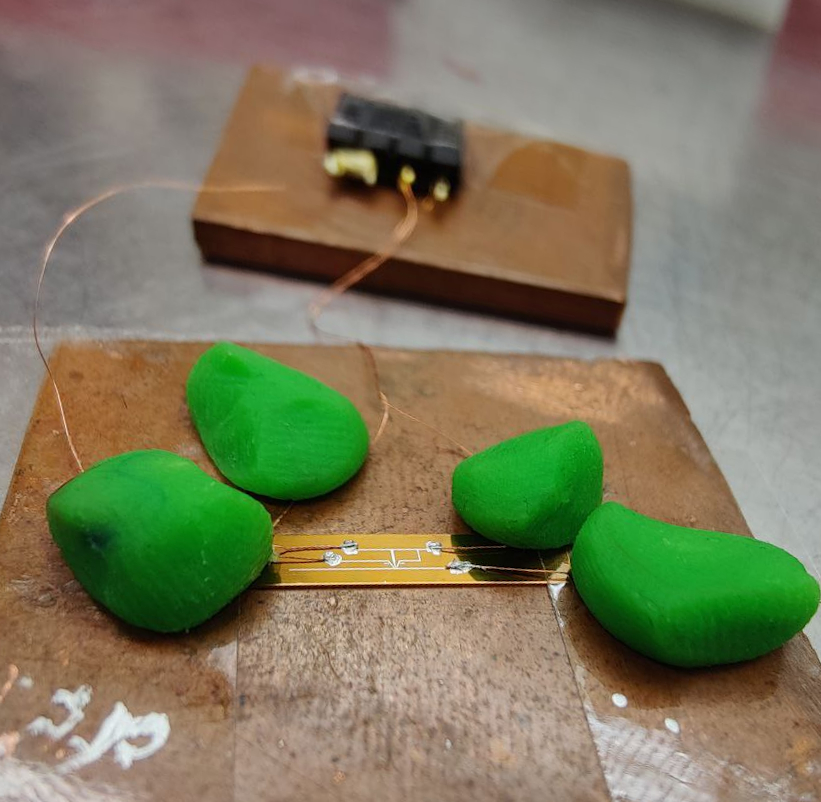
\includegraphics[width=.4\textwidth]{methods/sample/contacting/contacting.jpg}
            \caption{Example of a contacted sample, before adding strain relief.}
            \label{fig:methods:contacting}
        \end{wrapfigure}

        I position the wire ends on the sample pads with the help of modeling clay, as shown in Fig.~\ref{fig:methods:contacting}. Then, using a sharpened toothpick, I apply a small amount of silver paste to connect each wire to its pad. The viscosity of the silver paste is critical. If it is too fluid, shorts could form. If it is too viscous, it tends to remain on the toothpick instead of wetting the pad properly. In practice, paste collected from the lid after shaking the bottle works well. I transfer only enough paste to wet the pad. Afterward, I apply two-component epoxy as strain relief for the wires. Again, the viscosity is important. If I use the epoxy too soon after mixing, it continues to flow and could spread into unwanted areas. Because the interaction between epoxy and silver paste is not fully understood, I keep the two materials separate as much as possible. I test the epoxy on small trial dots and wait until it reaches a suitable consistency before applying it to the sample. I glue the two sides of the sample separately because the useful working window is fairly short.
        
        After mounting the sample in the cryostat, I scratch the shorting bridge with an engraving tool. I ensure proper grounding during this step and while closing the radiation shields by wearing a grounding bracelet. In dry conditions, I also increase the ambient humidity to reduce the risk of electrostatic discharge.

    \newpage
    %=========================================================
    \subsection*{Summary of Key Process Parameters}
    %=========================================================
    
        \begin{table}[!h]
            \centering
            \small
            \caption{Key process parameters used for sample preparation.}
            \label{tab:methods:sample_parameter}
            \vspace{1em}
            \begin{tabular}{ll}
                \hline
                Sacrificial layer   & Durimide 115A\\
                Spinning            & spread cycle: \qty{300}{\rpm} for \qty{30}{\second}\\
                                    & spin cycle: \qty{5000}{\rpm} for \qty{90}{\second}\\
                                    & ramp time: \qty{3}{\second}, \texttt{Program 3}\\
                Soft baking         & \qty{135}{\degreeCelsius} for \qty{5}{\minute} in convection oven\\
                Hard baking         & \qty{400}{\degreeCelsius} for \qty{30}{\minute} in vacuum oven\\

                \hline
                Spacing layer       & EL11 (MMA(8.5)MAA)\\
                Spinning            & spread cycle: \qty{500}{\rpm} for \qty{5}{\second}\\
                                    & spin cycle: \qty{2500}{\rpm} for \qty{90}{\second}\\
                                    & ramp time: \qty{3}{\second}, \texttt{Program 1}\\
                Soft baking         & \qty{150}{\degreeCelsius} for \qty{1}{\minute} on hot plate\\

                \hline
                Electron resist     & 950 A4 (PMMA)\\
                Spinning            & spread cycle: \qty{500}{\rpm} for \qty{5}{\second}\\
                                    & spin cycle: \qty{5000}{\rpm} for \qty{60}{\second}\\
                                    & ramp time: \qty{3}{\second}, \texttt{Program 2}\\
                Hard baking         & \qty{170}{\degreeCelsius} for \qty{30}{\minute} in convection oven\\

                \hline
                Exposure            & \texttt{Crossbeam} by Zeiss, \texttt{Elphy Plus} by Raith\\
                Settings            & \qty{10}{\kilo\volt} acceleration voltage, \qty{5}{\milli\meter} working distance,\\
                Aperture            & \qty{30}{\micro\meter} and \qty{120}{\micro\meter} aperture, high current,\\
                                    & \qty{155}{\micro\coulomb\per\centi\meter\squared} area dose\\
                Development         & \qty{25}{\second} in 1:3 MIBK:IPA\\
                                    & \qty{60}{\second} in IPA\\
                
                \hline
                Shadow evaporation  & First layer: \qty{60}{\nano\meter} Al at \qty{4}{\degree}\\
                                    & Oxidation: \qty{3.0(2)}{\milli\barunit} O\textsubscript{2} for \qty{3}{\minute}\\
                                    & Second layer: \qty{100}{\nano\meter} Al at \qty{34}{\degree}\\
                Lift-off            & \qtyrange{1}{3}{\hour} in acetone at \qty{60}{\degreeCelsius}\\

                \hline
                Reactive ion etching & \texttt{PlasmaPro 80} ICP RIE by Oxford Instruments\\
                                    & \texttt{mcbj sset v5 @ 100C}, see Table~\ref{tab:methods:rie_parameter}\\
                \hline
                Electrical contacting & \qty{90}{\micro\meter} insulated copper wire, silver paste as\\
                                    & electrical contact and epoxy as strain relief\\
            \end{tabular}
        \end{table}
